\noindent This supplement belongs to the main paper of the same title. It holds the material that did not fit the page limit: the live runtime and its experiments (Sections~\ref{sec:live} and~\ref{sec:livexp}), the multi-camera layer (Section~\ref{sec:system}), additional figures and tables, and per-seed results. References to ``the main paper'' point to the submission itself. Every number is generated from the same result files as in the main paper.

\section{Live Runtime}
\label{sec:live}
The live runtime turns the model into a process that reads two cameras and keeps running when they misbehave.

\paragraph{Capture}
Each camera runs in its own thread, stamps every frame with a monotonic time at the moment of capture, and writes it into a one-slot queue. A put replaces the frame waiting there and counts it as dropped, so a slow consumer never builds a backlog and latency cannot grow with time. A source that fails is reopened with backoff. Sources are a webcam index, an RTSP stream over TCP, or a replay of a recorded sequence at real speed with injected link faults: stalls, frozen frames, unplugs, random drops, delay and jitter.

\paragraph{Health monitor}
A monitor watches each camera from arrival times and pixels. It declares a camera stalled when no frame has arrived for \cfgStallIntervals{} nominal frame intervals, frozen when a downsampled frame has stayed nearly unchanged for \cfgFreezeFrames{} consecutive frames, black when the mean intensity is near zero, and saturated when a large share of pixels sits at the top of the range. Stalled, frozen and black cameras are \emph{down}, a saturated camera is \emph{degraded}, and others are \emph{ok}. The nominal rate is \cfgNominalFps{} frames per second.

\paragraph{Inference loop}
Each step takes the newest visible frame, waiting at most one frame interval, and the newest thermal frame without waiting, and reuses the last frame of a camera that has produced none. A camera that is down contributes a zero image and a zero sensor flag, which forces its reliability to zero everywhere, so the detector sees the failure as a stated fact rather than inferring it from a black picture. The gap between the timestamps of consecutive newest frames sets $\tau_t$ for the memory, and a gap longer than \cfgResetS{}\,s resets it. The model runs under half precision, followed by ByteTrack. Each step records inference time, end-to-end time from capture of the newest frame to the end of tracking, the time gap, the offset between the two camera timestamps, the health of each camera and the allocated GPU memory.

\paragraph{Summaries}
A run is summarised by throughput, median and 95th-percentile inference and end-to-end time, drift (the median end-to-end time over the last fifth of the run minus that over the first fifth), and growth in GPU memory. Fault handling is summarised by the delay from a fault's onset to the first \emph{down} status, the delay from its end to the first \emph{ok}, and the rate of false alarms.

\section{Live Runtime Experiments}
\label{sec:livexp}
This section tests the runtime of Section~\ref{sec:live} on the two properties a deployed system needs: that delay and memory stay bounded over a long run, and that a failing camera is noticed quickly and without false alarms. Recorded KAIST test sequences are replayed at real speed as the two cameras, so every run is repeatable and the faults are exact. The runtime uses CFFM-Net v2 trained on KAIST with the memory of the main paper and ByteTrack. It ran on the same \latLocalDevice{} as the latency measurements of the main paper; its inference times are higher than there because they are measured inside the running pipeline and include the memory, pre-processing and the tracker.

\subsection{Soak test}
\label{sec:soak}
Paired \cfgLatW{}$\times$\cfgLatH{} cameras ran at 30 frames per second for ten minutes (\livSoakThirtySeconds{}\,s) and at 20 frames per second for \cfgSoakShortSeconds{}\,s. A frame that the model cannot take is dropped at capture and never queued.

\begin{table}[t]
\centering
\caption{Live runtime on replayed KAIST sequences. Soak: paired cameras at the stated rate. Link faults: 20\,fps with a scripted cable pull, freeze and stall. Drift is the late minus the early median end-to-end delay. One run per row.}
\label{tab:live}
{\footnotesize\setlength{\tabcolsep}{4pt}
\adjustbox{max width=\linewidth}{\begin{tabular}{lcccc}
\toprule
& \multicolumn{2}{c}{Soak} & \multicolumn{2}{c}{Link faults} \\ \cmidrule(lr){2-3}\cmidrule(lr){4-5} Measure & 30 fps & 20 fps & Monitor on & Monitor off \\
\midrule
Run time (s) & \livSoakThirtySeconds & \livSoakTwentySeconds & \livFaultOnSeconds & \livFaultOffSeconds \\
Throughput (frames/s) & \livSoakThirtyFps & \livSoakTwentyFps & \livFaultOnFps & \livFaultOffFps \\
Capture drop (\%) & \livSoakThirtyDropPercent & \livSoakTwentyDropPercent & -- & -- \\
End-to-end median (ms) & \livSoakThirtyEndToEndMedianMs & \livSoakTwentyEndToEndMedianMs & \livFaultOnEndToEndMedianMs & \livFaultOffEndToEndMedianMs \\
End-to-end p95 (ms) & \livSoakThirtyEndToEndPNinetyFiveMs & \livSoakTwentyEndToEndPNinetyFiveMs & \livFaultOnEndToEndPNinetyFiveMs & \livFaultOffEndToEndPNinetyFiveMs \\
Inference median (ms) & \livSoakThirtyInferMedianMs & \livSoakTwentyInferMedianMs & \livFaultOnInferMedianMs & \livFaultOffInferMedianMs \\
Inference p95 (ms) & \livSoakThirtyInferPNinetyFiveMs & \livSoakTwentyInferPNinetyFiveMs & \livFaultOnInferPNinetyFiveMs & \livFaultOffInferPNinetyFiveMs \\
Drift (ms) & \livSoakThirtyDriftMs & \livSoakTwentyDriftMs & \livFaultOnDriftMs & \livFaultOffDriftMs \\
GPU memory growth (MB) & \livSoakThirtyGpuGrowthMb & \livSoakTwentyGpuGrowthMb & \livFaultOnGpuGrowthMb & \livFaultOffGpuGrowthMb \\
Miss rate, all frames (\%) & -- & -- & \livFaultOnMr & \livFaultOffMr \\
Camera reconnects & -- & -- & \livFaultOnReconnects & \livFaultOffReconnects \\
\bottomrule
\end{tabular}}}
\end{table}


Table~\ref{tab:live} gives the results. The stability criterion is met: over the ten-minute run the end-to-end delay drifts by \livSoakThirtyDriftMs{}\,ms and GPU memory changes by \livSoakThirtyGpuGrowthMb{}\,MB, so neither grows. The runtime is not real time at the camera rate on this hardware, however. At a nominal 30 frames per second it processes \livSoakThirtyFps{} and drops \livSoakThirtyDropPercent{}\,\% of the captured frames, and at 20 frames per second it processes \livSoakTwentyFps{} and drops \livSoakTwentyDropPercent{}\,\%. The median inference time with memory and tracking is \livSoakThirtyInferMedianMs{}\,ms and the median end-to-end delay \livSoakThirtyEndToEndMedianMs{}\,ms at 30 frames per second, with a 95th percentile of \livSoakThirtyEndToEndPNinetyFiveMs{}\,ms. The delay stays bounded because the capture drops frames rather than queueing them, which trades temporal resolution for latency. The shorter run drifts by \livSoakTwentyDriftMs{}\,ms, about eight percent of its median delay, and is too short to show whether that settles.

\subsection{Link faults and the stream monitor}
\label{sec:linkfaults}
A scripted run of \cfgLinkSeconds{}\,s at 20 frames per second applies three faults: the thermal cable pulled for \cfgUnplugSeconds{}\,s from second 20, the visible camera frozen for \cfgUnplugSeconds{}\,s from second 50, and the thermal stream stalled for \cfgStallSeconds{}\,s from second 80. Throughout, \cfgLinkDropPercent{}\,\% of frames are dropped at random and the thermal stream is delayed by \cfgLinkDelayMs{}\,ms. We repeat the run with the monitor feeding the sensor flags to the model (on) and with the monitor observing only (off).

\begin{table}[t]
\centering
\caption{Stream monitor timing for each scripted fault, with the monitor feeding the model (on) and only observing (off). Delays are seconds from onset or end of the fault to the first change of state.}
\label{tab:monitor}
{\footnotesize\setlength{\tabcolsep}{4pt}
\adjustbox{max width=\linewidth}{\begin{tabular}{lcccccc}
\toprule
& \multicolumn{2}{c}{Detect (s)} & \multicolumn{2}{c}{Recover (s)} & \multicolumn{2}{c}{False alarms (\%)} \\ \cmidrule(lr){2-3}\cmidrule(lr){4-5}\cmidrule(lr){6-7} Fault & On & Off & On & Off & On & Off \\
\midrule
Thermal unplugged, 6\,s & \livFaultOnUnpluggedDetectS & \livFaultOffUnpluggedDetectS & \livFaultOnUnpluggedRecoverS & \livFaultOffUnpluggedRecoverS & \livFaultOnUnpluggedFalseAlarmPercent & \livFaultOffUnpluggedFalseAlarmPercent \\
Visible frozen, 6\,s & \livFaultOnFrozenDetectS & \livFaultOffFrozenDetectS & \livFaultOnFrozenRecoverS & \livFaultOffFrozenRecoverS & \livFaultOnFrozenFalseAlarmPercent & \livFaultOffFrozenFalseAlarmPercent \\
Thermal stalled, 3\,s & \livFaultOnStalledDetectS & \livFaultOffStalledDetectS & \livFaultOnStalledRecoverS & \livFaultOffStalledRecoverS & \livFaultOnStalledFalseAlarmPercent & \livFaultOffStalledFalseAlarmPercent \\
\bottomrule
\end{tabular}}}
\end{table}


Table~\ref{tab:monitor} gives the monitor timing. A cable pull is flagged \livFaultOnUnpluggedDetectS{}\,s after onset and cleared \livFaultOnUnpluggedRecoverS{}\,s after the camera returns, a stall is flagged after \livFaultOnStalledDetectS{}\,s and cleared after \livFaultOnStalledRecoverS{}\,s, and a frozen visible camera is flagged after \livFaultOnFrozenDetectS{}\,s, which is longer because a freeze is recognised only after consecutive nearly identical frames and a replayed stream drops frames at random. The monitor is not free of false alarms: the thermal stream is marked down outside the scripted windows in \livFaultOnUnpluggedFalseAlarmPercent{}\,\% of records in the cable-pull measurement and \livFaultOnStalledFalseAlarmPercent{}\,\% in the stall measurement, which we attribute to the random drops and the added delay but did not test separately. The visible camera had none.

Feeding the flags to the model gives no measured accuracy benefit. The miss rate over all frames is \livFaultOnMr{}\,\% with the monitor on and \livFaultOffMr{}\,\% with it off, a difference of \livFaultMrChange{}\,points against the monitor, and throughput and delay are the same within a fraction of a frame (\livFaultOnFps{} against \livFaultOffFps{} frames per second). This is one run, the scripted faults cover only fifteen of the \cfgLinkSeconds{} seconds, and the memory-trained detector may already cope with a black thermal frame, in line with the flagged-versus-unflagged result of the main paper. We conclude that the monitor detects and clears link faults quickly, and that we have not shown that its flags improve detection. Both runs reopened the cameras \livFaultOnReconnects{} times.


\section{The Full System}
\label{sec:system}
The detector is one stage of a pipeline that runs from cameras to counts. Two paired cameras feed the live runtime of Section~\ref{sec:live}, whose monitor converts stream health into sensor flags. CFFM-Net with its Temporal State Memory produces detections, ByteTrack turns them into tracks, and records of latency, health and track state feed the analysis boards. A separate layer takes detections from several calibrated cameras and produces anonymous ground-plane tracks and aggregate analytics. This section describes that layer and reports its results.

\subsection{Multi-camera layer}
The multi-camera layer uses a plain RGB YOLO26-m detector, not CFFM-Net. WILDTRACK~\cite{chavdarova2018wildtrack} has \cfgCamViews{} synchronised, calibrated visible cameras and no thermal channel, so the layer demonstrates the system's last stage, from boxes to analytics, and provides no evidence about fusion. We evaluate the same layer with the detector zero-shot from COCO weights and fine-tuned on the training frames, which are exported as per-view person boxes. Frames are sampled every \cfgWtStep{} frames, and the frames from index \cfgWtTestFrom{} on are held out of the export.

\paragraph{From boxes to the ground plane}
Camera calibration gives a homography between the ground plane, in centimetres, and each image. The bottom centre of each person box is mapped to the ground, and points that fall outside the monitored area or whose back-projected ray misses the ground in front of the camera are discarded. Points from different cameras are merged by visibility-normalised voting. A candidate position is kept only if enough of the cameras that could see a person standing there did detect one near it, which avoids penalising people who stand in a blind spot of most cameras. Each candidate must also have enough support: the mean of the best nearby scores, normalised by the number of cameras that see the position, must exceed a threshold, and candidates closer than a minimum separation are suppressed in favour of the more confident. The merging radius is \camFusionFineTunedRadius{}\,cm for both detectors, the required fraction of visible cameras is \camFusionFineTunedMinRatio{}, and the score threshold is \camFusionZeroShotMinScore{} for the zero-shot detector and \camFusionFineTunedMinScore{} for the fine-tuned one.

\paragraph{Tracking and analytics}
Fused positions feed a constant-velocity tracker on the ground plane with Hungarian association, a gate of \cfgTrackGate{}\,cm, a track kept through \cfgTrackMiss{} missed frames, and confirmation after \cfgTrackHits{} hits. Identifiers are ephemeral and anonymous. The analytics are aggregate: counts per zone and in total, crossings of a line in each direction, dwell time per zone, and an occupancy map on a grid of \cfgGroundCell{}\,cm cells. As a privacy measure, the head region of every person box is blurred before any image is stored or displayed.

\subsection{Results}
Table~\ref{tab:multicam} reports detection, tracking and counting. Zero-shot, the detector has high precision (\camDetZeroShotPrecision{}\,\%) and low recall (\camDetZeroShotRecall{}\,\%), giving a MODA of \camDetZeroShotModa{}\,\%. These are the numbers of a detector that has never seen the viewpoint: it finds \camDetZeroShotTp{} people and misses \camDetZeroShotFn{}. Fine-tuning on the training frames lifts MODA to \camDetFineTunedModa{}\,\%, with recall \camDetFineTunedRecall{}\,\% and precision \camDetFineTunedPrecision{}\,\%, and cuts the misses to \camDetFineTunedFn{} at the price of more false positives (\camDetFineTunedFp{} against \camDetZeroShotFp{}). Localisation quality, MODP, is similar for the two, \camDetZeroShotModp{}\,\% and \camDetFineTunedModp{}\,\%.

On the ground-plane tracks the system reaches MOTA \camTrackMota{}\,\% and IDF1 \camTrackIdfOne{}\,\%, with \camTrackSwitches{} identity switches, and tracks \camTrackMostlyTracked{} of \camTrackUniqueObjects{} people for most of their presence. Counting is accurate enough to be useful: the mean absolute error of the total count is \camCountMae{} people on a mean of \camCountMeanPeople{} people per frame, a relative error of \camCountRelErr{}\,\%, and the error per zone ranges from \camCountZoneThreeMae{} to \camCountZoneTwoMae{} people. Crossings of the reference line number \camCrossBackward{} in one direction and \camCrossForward{} in the other. The busiest zone is the second, with \camDwellZoneTwoTracks{} tracks and a mean dwell of \camDwellZoneTwoMeanS{}\,s, against \camDwellZoneOneMeanS{}\,s in the first and \camDwellZoneThreeMeanS{}\,s in the third.

These results describe the multi-camera layer on RGB input. Tracking and counting run on the fine-tuned YOLO26-m detections. They say nothing about whether visible-thermal fusion improves analytics, which would require paired multi-camera thermal data that WILDTRACK lacks.

\begin{table}[t]
\centering
\caption{Multi-camera analytics. Detection uses zero-shot and fine-tuned YOLO26-m with ground-plane fusion; tracking and counting are reported once.}
\label{tab:multicam}
{\footnotesize\setlength{\tabcolsep}{4pt}
\adjustbox{max width=\linewidth}{\begin{tabular}{lcc}
\toprule
Measure & Zero-shot & Fine-tuned \\
\midrule
\multicolumn{3}{l}{\emph{Detection}} \\
MODA (\%) & \camDetZeroShotModa & \camDetFineTunedModa \\
MODP (\%) & \camDetZeroShotModp & \camDetFineTunedModp \\
Precision (\%) & \camDetZeroShotPrecision & \camDetFineTunedPrecision \\
Recall (\%) & \camDetZeroShotRecall & \camDetFineTunedRecall \\
True positives & \camDetZeroShotTp & \camDetFineTunedTp \\
False positives & \camDetZeroShotFp & \camDetFineTunedFp \\
False negatives & \camDetZeroShotFn & \camDetFineTunedFn \\
\midrule
\multicolumn{3}{l}{\emph{Tracking}} \\
MOTA (\%) & \multicolumn{2}{c}{\camTrackMota} \\
IDF1 (\%) & \multicolumn{2}{c}{\camTrackIdfOne} \\
ID switches & \multicolumn{2}{c}{\camTrackSwitches} \\
Mostly tracked of \camTrackUniqueObjects & \multicolumn{2}{c}{\camTrackMostlyTracked} \\
\midrule
\multicolumn{3}{l}{\emph{Counting}} \\
Count MAE (people) & \multicolumn{2}{c}{\camCountMae} \\
Relative error (\%) & \multicolumn{2}{c}{\camCountRelErr} \\
Zone one MAE & \multicolumn{2}{c}{\camCountZoneOneMae} \\
Zone two MAE & \multicolumn{2}{c}{\camCountZoneTwoMae} \\
Zone three MAE & \multicolumn{2}{c}{\camCountZoneThreeMae} \\
\bottomrule
\end{tabular}}}
\end{table}


\section{Additional Figures and Tables}
\label{sec:extra}
Figure~\ref{fig:scan} shows one step of the gated scan, Fig.~\ref{fig:tsm} the Temporal State Memory, Fig.~\ref{fig:trust} the share of fusion weight given to the thermal camera and Fig.~\ref{fig:hero} a trust map. For a round-one model the thermal share of the fusion weight moves in the expected direction with the brightness of the visible image: in the darkest LLVIP scenes it leans toward thermal and in the brightest M3FD scenes toward visible. The swing is small and the share stays close to one half everywhere, so the gate at round one is a mild prior and not a switch. Table~\ref{tab:scale} gives the size bands, Table~\ref{tab:ablation} every ablation variant, Table~\ref{tab:rounds} the round history and Table~\ref{tab:latency} the cost of every model on a \latLocalDevice{}, in half precision at batch one.

\begin{figure}[t]
\centering
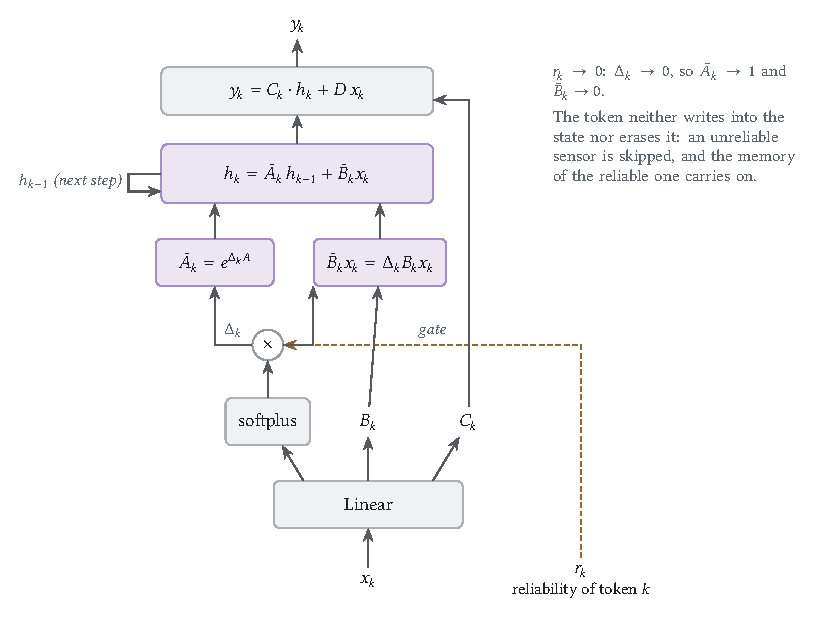
\includegraphics[width=0.8\columnwidth]{figures/fig_gated_scan.pdf}
\caption{One step of the gated scan. The reliability of the token's camera multiplies the step $\Delta_k$ before it enters the decay and the input term, so a reliability near zero leaves the state unchanged.}
\label{fig:scan}
\end{figure}

\begin{figure*}[t]
\centering
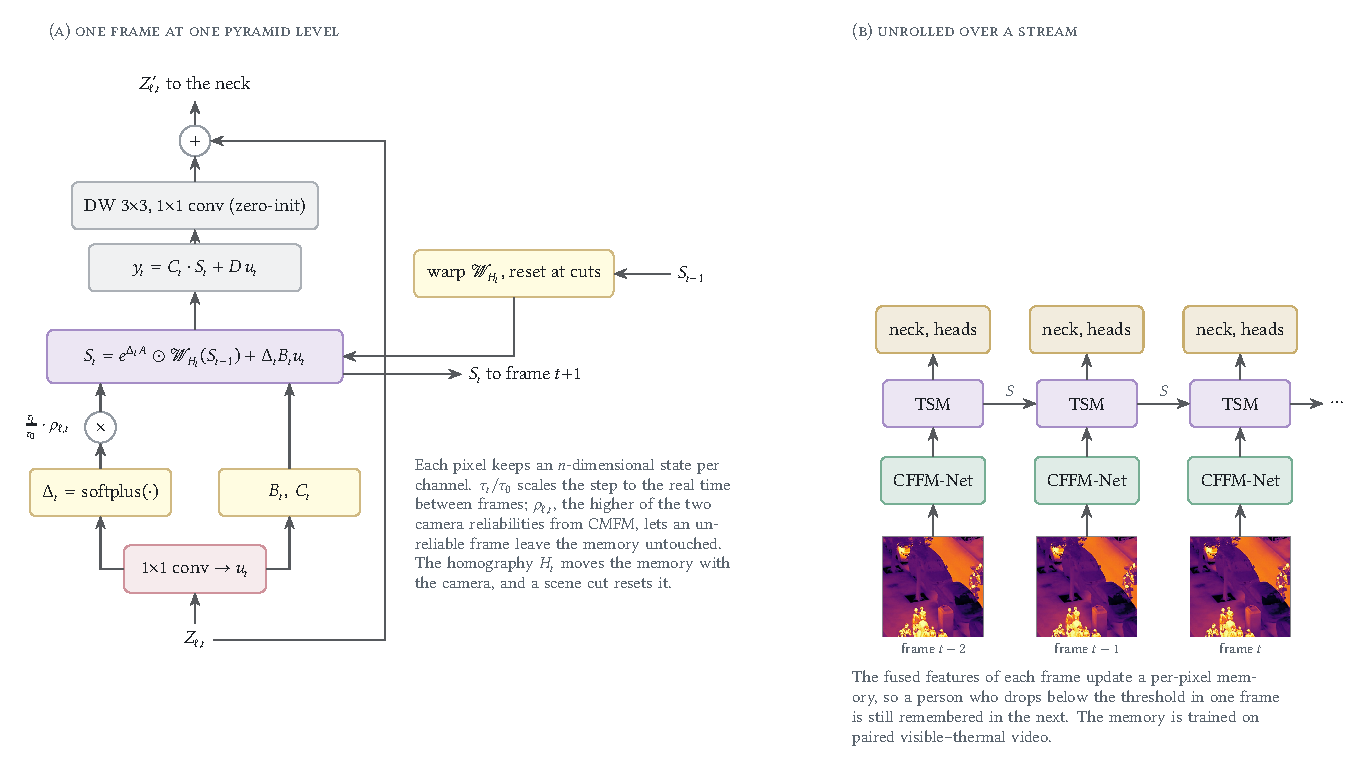
\includegraphics[width=0.82\textwidth]{figures/fig_tsm.pdf}
\caption{The Temporal State Memory. (a) One level at one frame: the step is scaled by elapsed time and by the camera reliability, and the previous state is warped by the frame-to-frame homography. (b) Unrolled over a stream, the memory sits between the fusion output and the neck.}
\label{fig:tsm}
\end{figure*}

\begin{figure*}[t]
\centering
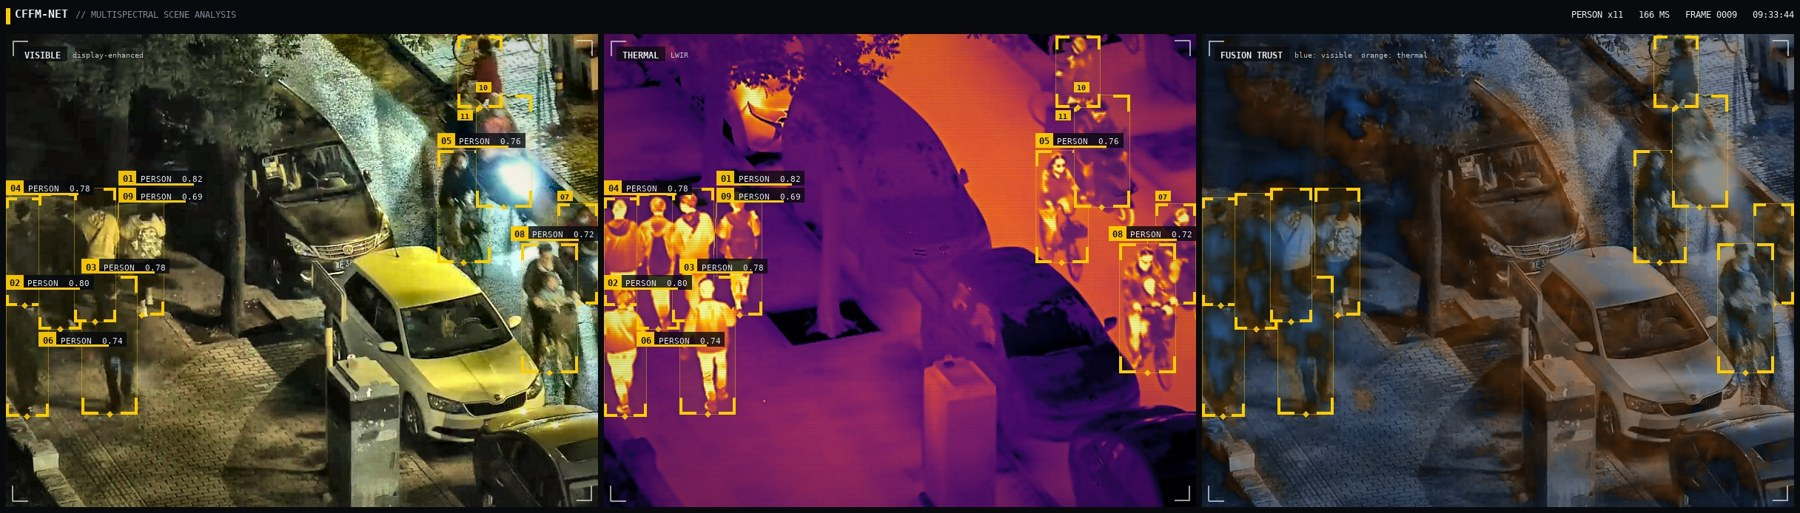
\includegraphics[width=0.9\textwidth]{figures/hero_llvip.jpg}
\caption{A LLVIP test pair as the round-one CFFM-Net sees it: visible with detections, thermal, and the fusion trust map in which blue marks visible and orange marks thermal weight.}
\label{fig:hero}
\end{figure*}

\begin{figure}[t]
\centering
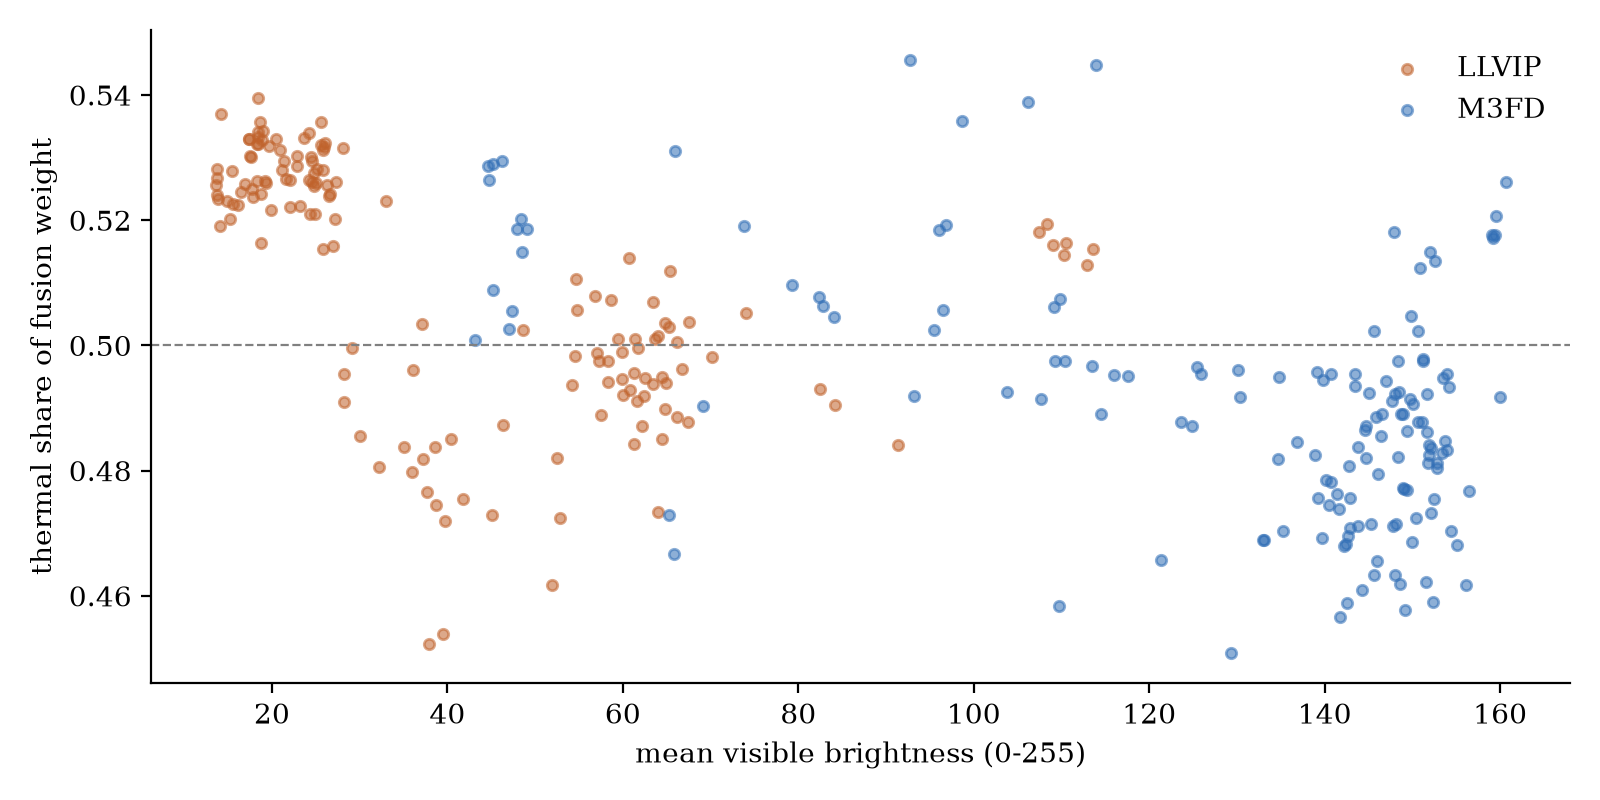
\includegraphics[width=\columnwidth]{figures/trust_vs_brightness.png}
\caption{Thermal share of the fusion weight against mean visible brightness for LLVIP and M3FD test images, with a round-one CFFM-Net. The dashed line marks an equal share.}
\label{fig:trust}
\end{figure}

\begin{table}[t]
\centering
\caption{Average precision by object size in percent, mean and sample std over three seeds, 80 epochs.}
\label{tab:scale}
{\footnotesize\setlength{\tabcolsep}{4pt}
\adjustbox{max width=\linewidth}{\begin{tabular}{lccc}
\toprule
Model & Small & Medium & Large \\
\midrule
\multicolumn{4}{l}{\emph{LLVIP}} \\
Concat, modality dropout & \resLlvipConcatMdMeanApSmall\,\ensuremath{\pm}\,\resLlvipConcatMdStdApSmall & \resLlvipConcatMdMeanApMedium\,\ensuremath{\pm}\,\resLlvipConcatMdStdApMedium & \resLlvipConcatMdMeanApLarge\,\ensuremath{\pm}\,\resLlvipConcatMdStdApLarge \\
CFFM-Net v2 & \resLlvipCffmVtwoMeanApSmall\,\ensuremath{\pm}\,\resLlvipCffmVtwoStdApSmall & \resLlvipCffmVtwoMeanApMedium\,\ensuremath{\pm}\,\resLlvipCffmVtwoStdApMedium & \resLlvipCffmVtwoMeanApLarge\,\ensuremath{\pm}\,\resLlvipCffmVtwoStdApLarge \\
Margin of v2 (pp) & \marLlvipVtwoVsConcatMdMeanApSmall\,\ensuremath{\pm}\,\marLlvipVtwoVsConcatMdStdApSmall & \marLlvipVtwoVsConcatMdMeanApMedium\,\ensuremath{\pm}\,\marLlvipVtwoVsConcatMdStdApMedium & \marLlvipVtwoVsConcatMdMeanApLarge\,\ensuremath{\pm}\,\marLlvipVtwoVsConcatMdStdApLarge \\
\midrule
\multicolumn{4}{l}{\emph{M3FD}} \\
Concat, modality dropout & \resMfdConcatMdMeanApSmall\,\ensuremath{\pm}\,\resMfdConcatMdStdApSmall & \resMfdConcatMdMeanApMedium\,\ensuremath{\pm}\,\resMfdConcatMdStdApMedium & \resMfdConcatMdMeanApLarge\,\ensuremath{\pm}\,\resMfdConcatMdStdApLarge \\
CFFM-Net v2 & \resMfdCffmVtwoMeanApSmall\,\ensuremath{\pm}\,\resMfdCffmVtwoStdApSmall & \resMfdCffmVtwoMeanApMedium\,\ensuremath{\pm}\,\resMfdCffmVtwoStdApMedium & \resMfdCffmVtwoMeanApLarge\,\ensuremath{\pm}\,\resMfdCffmVtwoStdApLarge \\
Margin of v2 (pp) & \marMfdVtwoVsConcatMdMeanApSmall\,\ensuremath{\pm}\,\marMfdVtwoVsConcatMdStdApSmall & \marMfdVtwoVsConcatMdMeanApMedium\,\ensuremath{\pm}\,\marMfdVtwoVsConcatMdStdApMedium & \marMfdVtwoVsConcatMdMeanApLarge\,\ensuremath{\pm}\,\marMfdVtwoVsConcatMdStdApLarge \\
\bottomrule
\end{tabular}}}
\end{table}

\begin{figure*}[t]
\centering
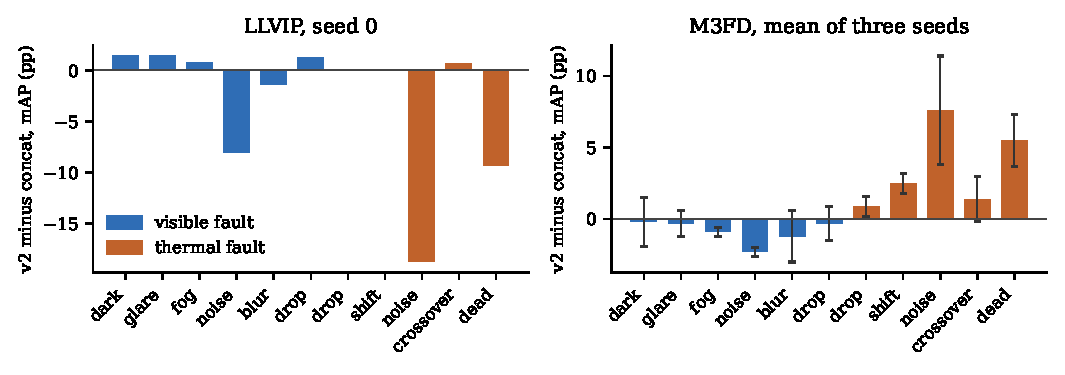
\includegraphics[width=0.78\textwidth]{figures/fig_fault_margin.pdf}
\caption{Margin of CFFM-Net v2 over the concat baseline for each fault at severity three, in mAP points, from the fault table of the main paper. Positive means v2 is ahead. LLVIP is one seed; M3FD shows the mean over three seeds with the sample standard deviation as an error bar.}
\label{fig:faultmargin}
\end{figure*}

\begin{table*}[t]
\centering
\caption{KAIST log-average miss rate in percent on the reasonable subset (lower is better). Published rows use the improved test annotations and the standard evaluation code and are copied from the cited papers. Our rows use the original annotations for training and testing, every 20th test frame and our own implementation of the protocol, so they are indicative only.}
\label{tab:sotakaist}
{\footnotesize\setlength{\tabcolsep}{4pt}
\adjustbox{max width=\linewidth}{\begin{tabular}{lllccc}
\toprule
Method & Detector & Train annotations & All & Day & Night \\
\midrule
AR-CNN~\cite{zhang2019arcnn} & VGG-16 & sanitized & 9.34 & 9.94 & 8.38 \\
MBNet~\cite{zhou2020mbnet} & ResNet-50 & AR-CNN improved & 8.13 & 8.28 & 7.86 \\
GAFF, original training~\cite{zhang2021gaff} & VGG-16 & original & 10.62 & 10.82 & 10.14 \\
GAFF, sanitized training~\cite{zhang2021gaff} & VGG-16 & sanitized & 6.48 & 8.35 & 3.46 \\
ICAFusion~\cite{shen2024icafusion} & YOLOv5, CSPDarknet53 & sanitized & 7.17 & 6.82 & 7.85 \\
MS-DETR~\cite{xing2024msdetr} & ResNet-50 & sanitized & 6.13 & 7.78 & 3.18 \\
TFDet~\cite{zhang2024tfdet} & VGG-16 & sanitized & 4.47 & 5.22 & 3.36 \\
\midrule
Concat baseline (this work) & YOLO26-n & original & \kstConcatAllMr & \kstConcatDayMr & \kstConcatNightMr \\
CFFM-Net v2 (this work) & YOLO26-n & original & \kstCffmAllMr & \kstCffmDayMr & \kstCffmNightMr \\
\bottomrule
\end{tabular}}}
\end{table*}

\begin{table}[t]
\centering
\caption{Ablation of mAP in percent. A dash marks a run that was not made.}
\label{tab:ablation}
{\footnotesize\setlength{\tabcolsep}{4pt}
\adjustbox{max width=\linewidth}{\begin{tabular}{lcc}
\toprule
Variant & LLVIP & M3FD \\
\midrule
\multicolumn{3}{l}{\emph{Round one, 30 epochs, seed 0}} \\
Two-stream concat & \resLlvipConcatPlainSeedZeroMap & \resMfdConcatPlainSeedZeroMap \\
CFFM-Net v1 & \resLlvipCffmVoneSeedZeroMap & \resMfdCffmVoneSeedZeroMap \\
v1, no gate & \resLlvipCffmVoneNogateSeedZeroMap & -- \\
v1, gated conv & \resLlvipCffmVoneGconvSeedZeroMap & -- \\
Concat + P2 head & \resLlvipConcatPtwoSeedZeroMap & -- \\
v1, no P2 head & \resLlvipCffmVoneNoptwoSeedZeroMap & -- \\
\midrule
\multicolumn{3}{l}{\emph{Rounds three and four, 80 epochs, seed 0}} \\
Concat, modality dropout & \resLlvipConcatMdSeedZeroMap & \resMfdConcatMdSeedZeroMap \\
CFFM-Net v2 & \resLlvipCffmVtwoSeedZeroMap & \resMfdCffmVtwoSeedZeroMap \\
Concat, fault training & \resLlvipConcatFtSeedZeroMap & \resMfdConcatFtSeedZeroMap \\
CFFM-Net v3 & \resLlvipCffmVthreeSeedZeroMap & \resMfdCffmVthreeSeedZeroMap \\
v3, no reliability branch & \resLlvipCffmVthreeNorelSeedZeroMap & \resMfdCffmVthreeNorelSeedZeroMap \\
\bottomrule
\end{tabular}}}
\end{table}

\begin{table}[t]
\centering
\caption{Round history: mAP margin of CFFM-Net over its control in percentage points.}
\label{tab:rounds}
{\footnotesize\setlength{\tabcolsep}{4pt}
\adjustbox{max width=\linewidth}{\begin{tabular}{p{0.6\columnwidth}cc}
\toprule
Comparison & LLVIP & M3FD \\
\midrule
Round one, v1 against concat (30 epochs) & \marLlvipVoneVsConcatPlainSeedZeroMap & \marMfdVoneVsConcatPlainSeedZeroMap \\
Head control, v1 without P2 against concat with P2 & \marLlvipVoneNoptwoVsConcatPtwoSeedZeroMap & -- \\
Round three, v2 against concat (seed 0) & \marLlvipVtwoVsConcatMdSeedZeroMap & \marMfdVtwoVsConcatMdSeedZeroMap \\
Round three, v2 against concat (three-seed mean) & \marLlvipVtwoVsConcatMdMeanMap & \marMfdVtwoVsConcatMdMeanMap \\
Round four, v3 against fault-trained concat & \marLlvipVthreeVsConcatFtSeedZeroMap & \marMfdVthreeVsConcatFtSeedZeroMap \\
Round four, v3 against v3 without reliability branch & \marLlvipVthreeVsVthreeNorelSeedZeroMap & \marMfdVthreeVsVthreeNorelSeedZeroMap \\
Round four, v3 against v2 & \marLlvipVthreeVsVtwoSeedZeroMap & \marMfdVthreeVsVtwoSeedZeroMap \\
\bottomrule
\end{tabular}}}
\end{table}

\begin{table}[t]
\centering
\caption{Parameters (millions), GFLOPs and latency (ms) on a \latLocalDevice{}, half precision, batch one, \cfgLatW{}$\times$\cfgLatH{} input, median and 95th percentile per image over \cfgLatIters{} timed iterations after \cfgLatWarmup{} warm-up iterations, on an otherwise idle GPU.}
\label{tab:latency}
{\footnotesize\setlength{\tabcolsep}{4pt}
\adjustbox{max width=\linewidth}{\begin{tabular}{lrrrr}
\toprule
Model & Params & GFLOPs & Median & p95 \\
\midrule
YOLO26-n thermal only & \latLocalYoloThmParamsM & \latLocalYoloThmGflops & \latLocalYoloThmMedianMs & \latLocalYoloThmPNinetyFiveMs \\
Concat, modality dropout & \latLocalConcatMdParamsM & \latLocalConcatMdGflops & \latLocalConcatMdMedianMs & \latLocalConcatMdPNinetyFiveMs \\
Concat, fault training & \latLocalConcatFtParamsM & \latLocalConcatFtGflops & \latLocalConcatFtMedianMs & \latLocalConcatFtPNinetyFiveMs \\
CFFM-Net v2 & \latLocalVtwoParamsM & \latLocalVtwoGflops & \latLocalVtwoMedianMs & \latLocalVtwoPNinetyFiveMs \\
v3, no reliability branch & \latLocalVthreeNorelParamsM & \latLocalVthreeNorelGflops & \latLocalVthreeNorelMedianMs & \latLocalVthreeNorelPNinetyFiveMs \\
CFFM-Net v3 & \latLocalVthreeParamsM & \latLocalVthreeGflops & \latLocalVthreeMedianMs & \latLocalVthreePNinetyFiveMs \\
\midrule
v2 over concat, ratio & \latLocalRatioParams & \latLocalRatioGflops & \latLocalRatioMedian & \latLocalRatioPNinetyFive \\
\bottomrule
\end{tabular}}}
\end{table}


\section{Per-seed results}
\label{app:seeds}
Table~\ref{tab:seeds} lists every run behind the headline comparison, with the mean and sample standard deviation over seeds. Table~\ref{tab:seedmargin} gives the per-seed mAP margin of v2 over the concat baseline, which is the quantity averaged in the main paper.

\begin{table*}[t]
\centering
\caption{Per-seed accuracy in percent, 80 epochs. The last three columns are COCO size bands.}
\label{tab:seeds}
{\footnotesize\setlength{\tabcolsep}{4.5pt}
\adjustbox{max width=\linewidth}{\begin{tabular}{llcccccccc}
\toprule
Dataset & Model & Seed & mAP & mAP$_{50}$ & Precision & Recall & Small & Medium & Large \\
\midrule
LLVIP & Concat, modality dropout & 0 & \resLlvipConcatMdSeedZeroMap & \resLlvipConcatMdSeedZeroMapFifty & \resLlvipConcatMdSeedZeroPrecision & \resLlvipConcatMdSeedZeroRecall & \resLlvipConcatMdSeedZeroApSmall & \resLlvipConcatMdSeedZeroApMedium & \resLlvipConcatMdSeedZeroApLarge \\
 &  & 1 & \resLlvipConcatMdSeedOneMap & \resLlvipConcatMdSeedOneMapFifty & \resLlvipConcatMdSeedOnePrecision & \resLlvipConcatMdSeedOneRecall & \resLlvipConcatMdSeedOneApSmall & \resLlvipConcatMdSeedOneApMedium & \resLlvipConcatMdSeedOneApLarge \\
 &  & 2 & \resLlvipConcatMdSeedTwoMap & \resLlvipConcatMdSeedTwoMapFifty & \resLlvipConcatMdSeedTwoPrecision & \resLlvipConcatMdSeedTwoRecall & \resLlvipConcatMdSeedTwoApSmall & \resLlvipConcatMdSeedTwoApMedium & \resLlvipConcatMdSeedTwoApLarge \\
& \emph{mean $\pm$ std} & & \resLlvipConcatMdMeanMap\,\ensuremath{\pm}\,\resLlvipConcatMdStdMap & \resLlvipConcatMdMeanMapFifty\,\ensuremath{\pm}\,\resLlvipConcatMdStdMapFifty & \resLlvipConcatMdMeanPrecision\,\ensuremath{\pm}\,\resLlvipConcatMdStdPrecision & \resLlvipConcatMdMeanRecall\,\ensuremath{\pm}\,\resLlvipConcatMdStdRecall & \resLlvipConcatMdMeanApSmall\,\ensuremath{\pm}\,\resLlvipConcatMdStdApSmall & \resLlvipConcatMdMeanApMedium\,\ensuremath{\pm}\,\resLlvipConcatMdStdApMedium & \resLlvipConcatMdMeanApLarge\,\ensuremath{\pm}\,\resLlvipConcatMdStdApLarge \\
 & CFFM-Net v2 & 0 & \resLlvipCffmVtwoSeedZeroMap & \resLlvipCffmVtwoSeedZeroMapFifty & \resLlvipCffmVtwoSeedZeroPrecision & \resLlvipCffmVtwoSeedZeroRecall & \resLlvipCffmVtwoSeedZeroApSmall & \resLlvipCffmVtwoSeedZeroApMedium & \resLlvipCffmVtwoSeedZeroApLarge \\
 &  & 1 & \resLlvipCffmVtwoSeedOneMap & \resLlvipCffmVtwoSeedOneMapFifty & \resLlvipCffmVtwoSeedOnePrecision & \resLlvipCffmVtwoSeedOneRecall & \resLlvipCffmVtwoSeedOneApSmall & \resLlvipCffmVtwoSeedOneApMedium & \resLlvipCffmVtwoSeedOneApLarge \\
 &  & 2 & \resLlvipCffmVtwoSeedTwoMap & \resLlvipCffmVtwoSeedTwoMapFifty & \resLlvipCffmVtwoSeedTwoPrecision & \resLlvipCffmVtwoSeedTwoRecall & \resLlvipCffmVtwoSeedTwoApSmall & \resLlvipCffmVtwoSeedTwoApMedium & \resLlvipCffmVtwoSeedTwoApLarge \\
& \emph{mean $\pm$ std} & & \resLlvipCffmVtwoMeanMap\,\ensuremath{\pm}\,\resLlvipCffmVtwoStdMap & \resLlvipCffmVtwoMeanMapFifty\,\ensuremath{\pm}\,\resLlvipCffmVtwoStdMapFifty & \resLlvipCffmVtwoMeanPrecision\,\ensuremath{\pm}\,\resLlvipCffmVtwoStdPrecision & \resLlvipCffmVtwoMeanRecall\,\ensuremath{\pm}\,\resLlvipCffmVtwoStdRecall & \resLlvipCffmVtwoMeanApSmall\,\ensuremath{\pm}\,\resLlvipCffmVtwoStdApSmall & \resLlvipCffmVtwoMeanApMedium\,\ensuremath{\pm}\,\resLlvipCffmVtwoStdApMedium & \resLlvipCffmVtwoMeanApLarge\,\ensuremath{\pm}\,\resLlvipCffmVtwoStdApLarge \\
\midrule
M3FD & Concat, modality dropout & 0 & \resMfdConcatMdSeedZeroMap & \resMfdConcatMdSeedZeroMapFifty & \resMfdConcatMdSeedZeroPrecision & \resMfdConcatMdSeedZeroRecall & \resMfdConcatMdSeedZeroApSmall & \resMfdConcatMdSeedZeroApMedium & \resMfdConcatMdSeedZeroApLarge \\
 &  & 1 & \resMfdConcatMdSeedOneMap & \resMfdConcatMdSeedOneMapFifty & \resMfdConcatMdSeedOnePrecision & \resMfdConcatMdSeedOneRecall & \resMfdConcatMdSeedOneApSmall & \resMfdConcatMdSeedOneApMedium & \resMfdConcatMdSeedOneApLarge \\
 &  & 2 & \resMfdConcatMdSeedTwoMap & \resMfdConcatMdSeedTwoMapFifty & \resMfdConcatMdSeedTwoPrecision & \resMfdConcatMdSeedTwoRecall & \resMfdConcatMdSeedTwoApSmall & \resMfdConcatMdSeedTwoApMedium & \resMfdConcatMdSeedTwoApLarge \\
& \emph{mean $\pm$ std} & & \resMfdConcatMdMeanMap\,\ensuremath{\pm}\,\resMfdConcatMdStdMap & \resMfdConcatMdMeanMapFifty\,\ensuremath{\pm}\,\resMfdConcatMdStdMapFifty & \resMfdConcatMdMeanPrecision\,\ensuremath{\pm}\,\resMfdConcatMdStdPrecision & \resMfdConcatMdMeanRecall\,\ensuremath{\pm}\,\resMfdConcatMdStdRecall & \resMfdConcatMdMeanApSmall\,\ensuremath{\pm}\,\resMfdConcatMdStdApSmall & \resMfdConcatMdMeanApMedium\,\ensuremath{\pm}\,\resMfdConcatMdStdApMedium & \resMfdConcatMdMeanApLarge\,\ensuremath{\pm}\,\resMfdConcatMdStdApLarge \\
 & CFFM-Net v2 & 0 & \resMfdCffmVtwoSeedZeroMap & \resMfdCffmVtwoSeedZeroMapFifty & \resMfdCffmVtwoSeedZeroPrecision & \resMfdCffmVtwoSeedZeroRecall & \resMfdCffmVtwoSeedZeroApSmall & \resMfdCffmVtwoSeedZeroApMedium & \resMfdCffmVtwoSeedZeroApLarge \\
 &  & 1 & \resMfdCffmVtwoSeedOneMap & \resMfdCffmVtwoSeedOneMapFifty & \resMfdCffmVtwoSeedOnePrecision & \resMfdCffmVtwoSeedOneRecall & \resMfdCffmVtwoSeedOneApSmall & \resMfdCffmVtwoSeedOneApMedium & \resMfdCffmVtwoSeedOneApLarge \\
 &  & 2 & \resMfdCffmVtwoSeedTwoMap & \resMfdCffmVtwoSeedTwoMapFifty & \resMfdCffmVtwoSeedTwoPrecision & \resMfdCffmVtwoSeedTwoRecall & \resMfdCffmVtwoSeedTwoApSmall & \resMfdCffmVtwoSeedTwoApMedium & \resMfdCffmVtwoSeedTwoApLarge \\
& \emph{mean $\pm$ std} & & \resMfdCffmVtwoMeanMap\,\ensuremath{\pm}\,\resMfdCffmVtwoStdMap & \resMfdCffmVtwoMeanMapFifty\,\ensuremath{\pm}\,\resMfdCffmVtwoStdMapFifty & \resMfdCffmVtwoMeanPrecision\,\ensuremath{\pm}\,\resMfdCffmVtwoStdPrecision & \resMfdCffmVtwoMeanRecall\,\ensuremath{\pm}\,\resMfdCffmVtwoStdRecall & \resMfdCffmVtwoMeanApSmall\,\ensuremath{\pm}\,\resMfdCffmVtwoStdApSmall & \resMfdCffmVtwoMeanApMedium\,\ensuremath{\pm}\,\resMfdCffmVtwoStdApMedium & \resMfdCffmVtwoMeanApLarge\,\ensuremath{\pm}\,\resMfdCffmVtwoStdApLarge \\
\bottomrule
\end{tabular}}}
\end{table*}

\begin{table}[t]
\centering
\caption{Per-seed mAP margin of CFFM-Net v2 over the concat baseline, in percentage points.}
\label{tab:seedmargin}
{\footnotesize\setlength{\tabcolsep}{6pt}
\adjustbox{max width=\linewidth}{\begin{tabular}{lccc}
\toprule
Dataset & Seed 0 & Seed 1 & Seed 2 \\
\midrule
LLVIP & \marLlvipVtwoVsConcatMdSeedZeroMap & \marLlvipVtwoVsConcatMdSeedOneMap & \marLlvipVtwoVsConcatMdSeedTwoMap \\
M3FD & \marMfdVtwoVsConcatMdSeedZeroMap & \marMfdVtwoVsConcatMdSeedOneMap & \marMfdVtwoVsConcatMdSeedTwoMap \\
\bottomrule
\end{tabular}}}
\end{table}

\section{Fine size bands on M3FD}
\label{app:bands}
Table~\ref{tab:bands} gives the finer size bands behind the main paper.

\begin{table}[t]
\centering
\caption{M3FD average precision in the finer size bands, percent, per seed and as mean and sample standard deviation.}
\label{tab:bands}
{\footnotesize\setlength{\tabcolsep}{3.5pt}
\adjustbox{max width=\linewidth}{\begin{tabular}{llccc}
\toprule
Model & Seed & Very tiny & Tiny & Small \\
\midrule
Concat, modality dropout & 0 & \resMfdConcatMdSeedZeroApBandVeryTiny & \resMfdConcatMdSeedZeroApBandTiny & \resMfdConcatMdSeedZeroApBandSmall \\
 & 1 & \resMfdConcatMdSeedOneApBandVeryTiny & \resMfdConcatMdSeedOneApBandTiny & \resMfdConcatMdSeedOneApBandSmall \\
 & 2 & \resMfdConcatMdSeedTwoApBandVeryTiny & \resMfdConcatMdSeedTwoApBandTiny & \resMfdConcatMdSeedTwoApBandSmall \\
& \emph{mean $\pm$ std} & \resMfdConcatMdMeanApBandVeryTiny\,\ensuremath{\pm}\,\resMfdConcatMdStdApBandVeryTiny & \resMfdConcatMdMeanApBandTiny\,\ensuremath{\pm}\,\resMfdConcatMdStdApBandTiny & \resMfdConcatMdMeanApBandSmall\,\ensuremath{\pm}\,\resMfdConcatMdStdApBandSmall \\
\midrule
CFFM-Net v2 & 0 & \resMfdCffmVtwoSeedZeroApBandVeryTiny & \resMfdCffmVtwoSeedZeroApBandTiny & \resMfdCffmVtwoSeedZeroApBandSmall \\
 & 1 & \resMfdCffmVtwoSeedOneApBandVeryTiny & \resMfdCffmVtwoSeedOneApBandTiny & \resMfdCffmVtwoSeedOneApBandSmall \\
 & 2 & \resMfdCffmVtwoSeedTwoApBandVeryTiny & \resMfdCffmVtwoSeedTwoApBandTiny & \resMfdCffmVtwoSeedTwoApBandSmall \\
& \emph{mean $\pm$ std} & \resMfdCffmVtwoMeanApBandVeryTiny\,\ensuremath{\pm}\,\resMfdCffmVtwoStdApBandVeryTiny & \resMfdCffmVtwoMeanApBandTiny\,\ensuremath{\pm}\,\resMfdCffmVtwoStdApBandTiny & \resMfdCffmVtwoMeanApBandSmall\,\ensuremath{\pm}\,\resMfdCffmVtwoStdApBandSmall \\
\bottomrule
\end{tabular}}}
\end{table}

\section{Degradation probe of the round-one models}
\label{app:probe}
Table~\ref{tab:probe} gives the LLVIP degradation probe that preceded the fault benchmark. It uses the round-one models at \cfgEpochsPilot{} epochs and one seed.

\begin{table}[t]
\centering
\caption{Degradation probe on LLVIP, mAP in percent, round-one models (30 epochs, seed 0).}
\label{tab:probe}
{\footnotesize\setlength{\tabcolsep}{4pt}
\adjustbox{max width=\linewidth}{\begin{tabular}{lccc}
\toprule
Condition & v1 & v1, no gate & Concat \\
\midrule
Clean & \prbLlvipCffmVoneCleanMap & \prbLlvipCffmVoneNogateCleanMap & \prbLlvipConcatPlainCleanMap \\
Visible dark & \prbLlvipCffmVoneVisibleDarkMap & \prbLlvipCffmVoneNogateVisibleDarkMap & \prbLlvipConcatPlainVisibleDarkMap \\
Visible drop & \prbLlvipCffmVoneVisibleDropMap & \prbLlvipCffmVoneNogateVisibleDropMap & \prbLlvipConcatPlainVisibleDropMap \\
Visible drop, flagged & \prbLlvipCffmVoneVisibleDropFlaggedMap & \prbLlvipCffmVoneNogateVisibleDropFlaggedMap & \prbLlvipConcatPlainVisibleDropFlaggedMap \\
Thermal drop & \prbLlvipCffmVoneThermalDropMap & \prbLlvipCffmVoneNogateThermalDropMap & \prbLlvipConcatPlainThermalDropMap \\
Thermal drop, flagged & \prbLlvipCffmVoneThermalDropFlaggedMap & \prbLlvipCffmVoneNogateThermalDropFlaggedMap & \prbLlvipConcatPlainThermalDropFlaggedMap \\
Thermal shift 4 px & \prbLlvipCffmVoneThermalShiftFourMap & \prbLlvipCffmVoneNogateThermalShiftFourMap & \prbLlvipConcatPlainThermalShiftFourMap \\
Thermal shift 8 px & \prbLlvipCffmVoneThermalShiftEightMap & \prbLlvipCffmVoneNogateThermalShiftEightMap & \prbLlvipConcatPlainThermalShiftEightMap \\
Thermal shift 16 px & \prbLlvipCffmVoneThermalShiftSixteenMap & \prbLlvipCffmVoneNogateThermalShiftSixteenMap & \prbLlvipConcatPlainThermalShiftSixteenMap \\
\bottomrule
\end{tabular}}}
\end{table}

